\documentclass[class=article,crop=false]{standalone}
\usepackage[subpreambles=true]{standalone}
\begin{document}
\lecture


\begin{figure}[h!]
	\centering
	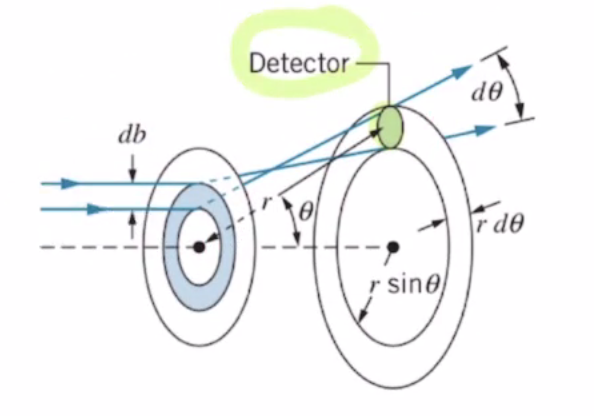
\includegraphics[width=.4\linewidth]{./Images/rdetector.png}
	\caption{Setup 3}
\end{figure}
\begin{result}[Rutherford Scattering Formula]
	Determine the probability for a projectile to be scattered at an angle $\theta$. \\
	From the fraction of projectiles scattered at angles greater than angle $\theta$, we can determine the fraction scattered into a small angular region from $\theta$ to $d\theta$.
	
	$$ f = nt\pi b^2 $$
	Fraction scattered into region:
	$$ df = nt\pi b db $$
	Impact parameter (b) related to scattering angle $\theta$:
	$$ b = \frac{zZ}{2K} \cdot \frac{e^2}{4\pi \epsilon_0} cot(\theta/2) $$
	Then we can differentiate b to express df with respect to d$\theta$.\\
	The fraction scattered into a small angular region (df) is scattered into a ring with area dA:
	$$ dA = (2\pi r sin\theta)*rd\theta $$
	The probability per unit area is the fraction scattered per unit area:
	$$ N(\theta) = \frac{|df|}{dA} = \frac{nt}{4r^2} \cdot (\frac{zZ}{2k})^2 \cdot (\frac{e^2}{4\pi \epsilon_0})^2 \cdot \frac{1}{sin^4(\theta/2)} $$
	Where\\
	n: number of nuclei per unit volume\\
	t: thickness of film\\
	r: distance between detector and nucleus\\
	z, Z: electric charges of projectile, nucleus\\
	K: kinetic energy\\
	$\theta$: scattering angle
\end{result}
These predictions were extensively tested by his Ph.D students, and confirmed.

\subsection{Line Spectra}
In the late 19th century, pure chemical elements were observed to produce unique wavelengths of light when burned. But not \emph{why}.

\begin{figure}[h!]
	\centering
	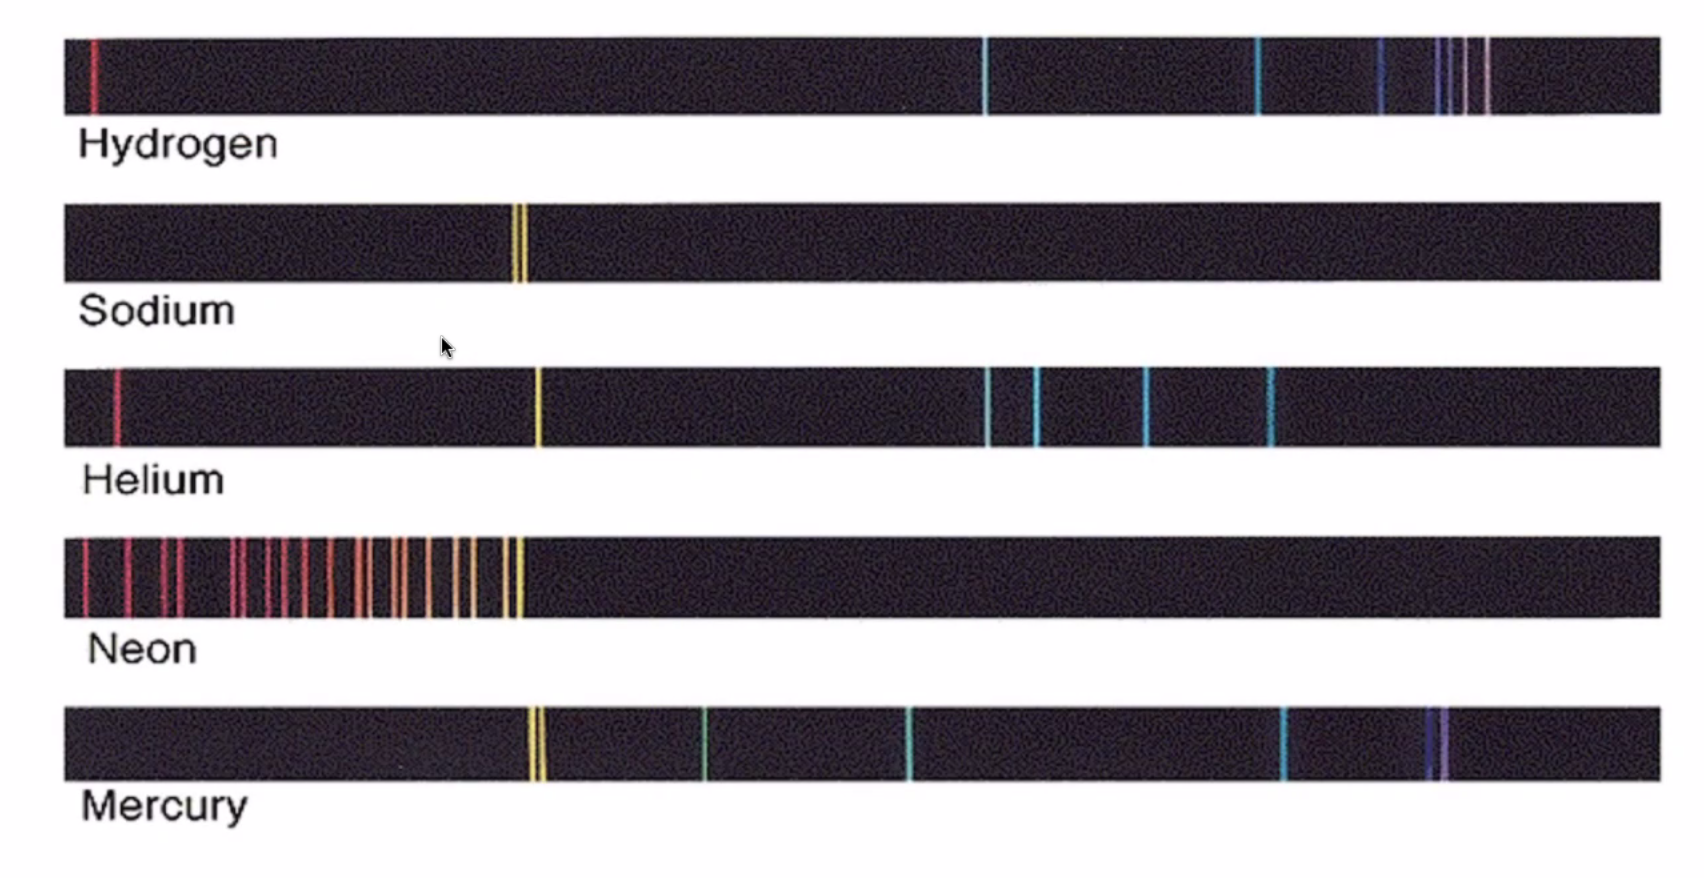
\includegraphics[width=.6\linewidth]{./Images/spectrums.png}
	\caption{Setup 3}
\end{figure}
Atoms can emit and absorb electromagnetic radiation. There can be either a continuous or discrete spectra (line spectra).

\begin{figure}[h!]
	\centering
	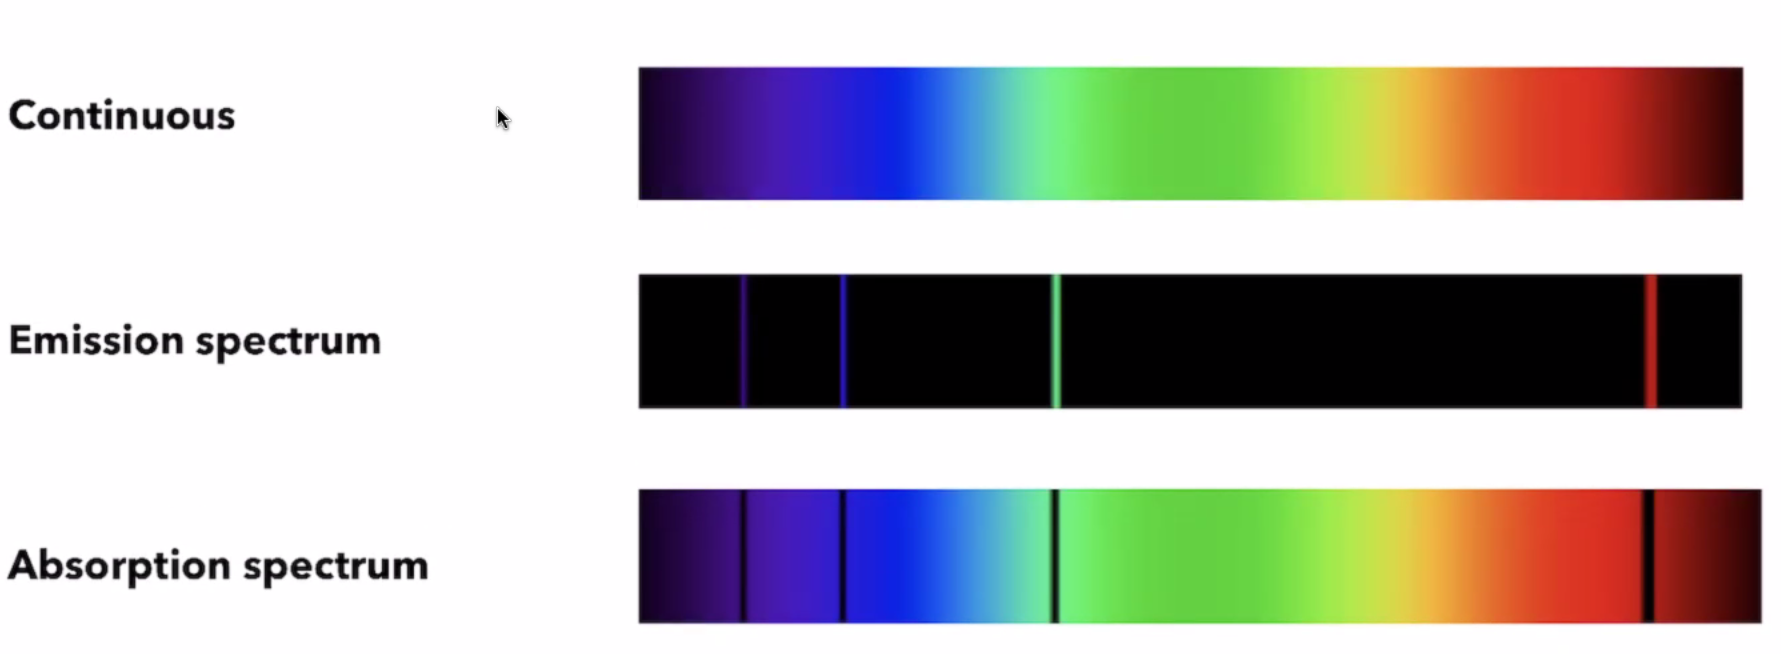
\includegraphics[width=.6\linewidth]{./Images/emission.png}
	\caption{Setup 3}
\end{figure}
Absorpion spectra generally correspond to many but \emph{not all} lines seen in emission spectra!\\

\subsubsection{Experimentally}
Emission spectra - Electric discharge created inside a tube containing a vaporized element.\\
Absorption spectra - Continuous spectrum of light sent through a vaporized element.
\begin{figure}[h!]
	\centering
	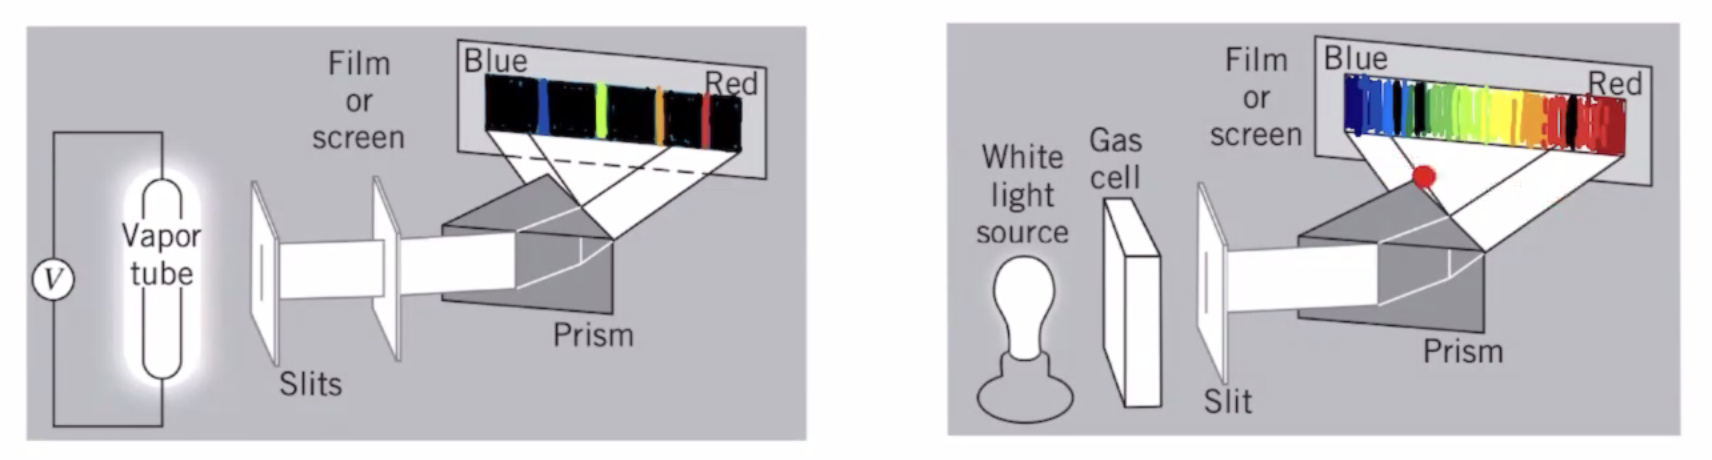
\includegraphics[width=.7\linewidth]{./Images/em_abs.png}
	\caption{Setup 3}
\end{figure}

\begin{figure}[h]
	\centering
	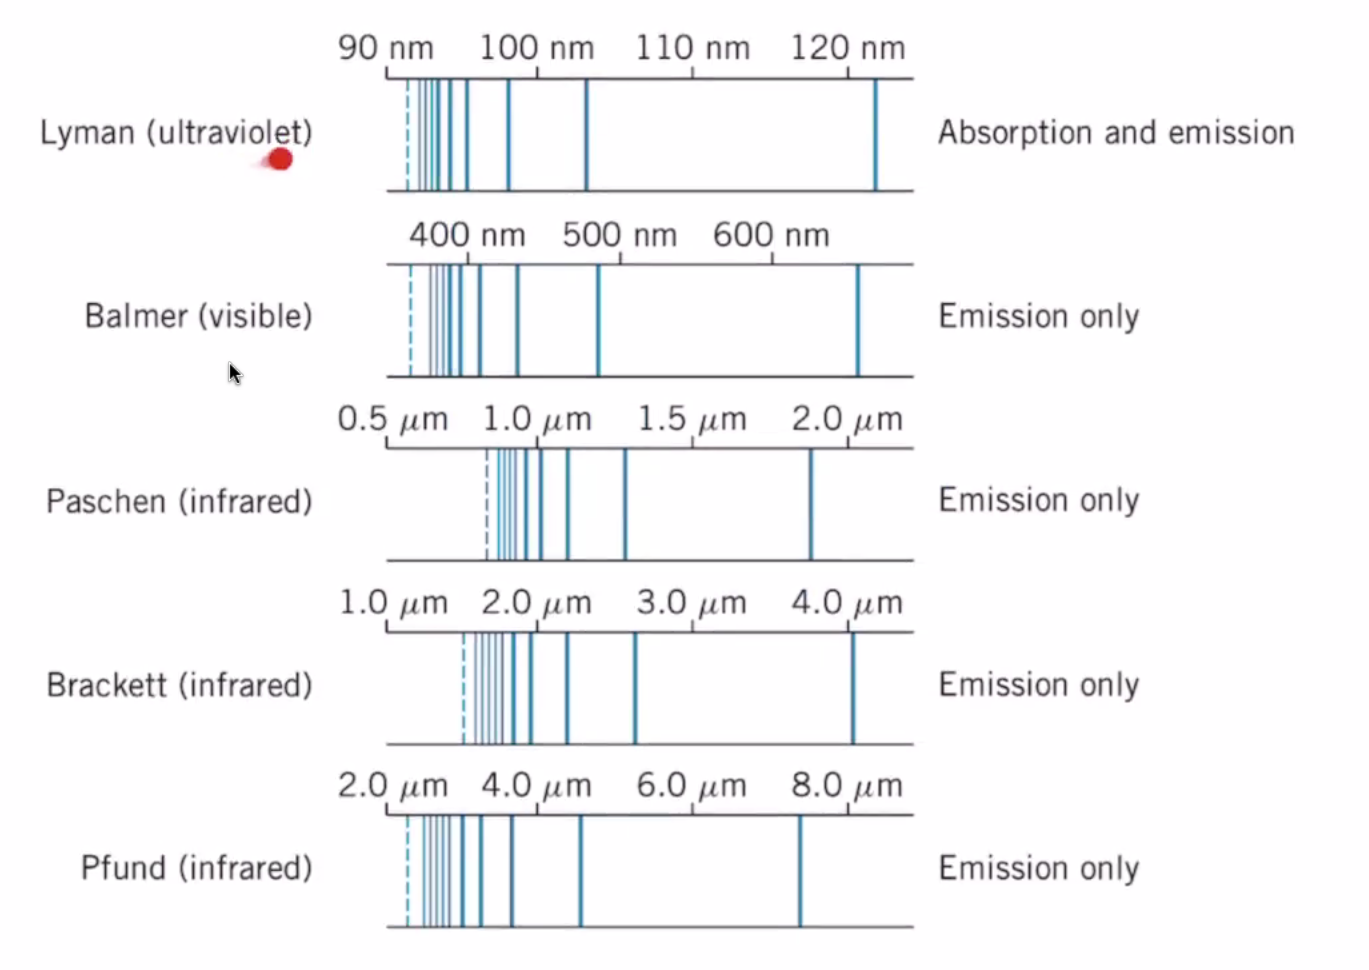
\includegraphics[width=.7\linewidth]{./Images/em_only.png}
	\caption{Wavelengths of various spectra}
\end{figure}

\subsubsection{Balmer Series}
1885 school teacher showed (basically from trial and error) that the wavelengths of the hydrogen emission lines in the visible region could be calculated as:\\
$$ \lambda = (364.5 nm)\cdot \frac{n^2}{n^2-4} $$
where n = 3, 4, 5, 6...\\

\begin{result}[General Hydrogen Spectra]
	Soon a more general formula describing all lines was discovered.
	$$ \lambda = \lambda_{limit} \frac{n^2}{n^2 - n_0^2} $$
	For n = $n_0 + 1, n_0 + 2, n_0 + 4, n_0 + 4 ....$
	$\lambda_{limit}$: wavelength of each series limit $(n \rightarrow \infty)$.
	$n_1 = 1$: Lyman Series
	$n_2 = 1$: Balmer Series
	$n_3 = 1$: Paschem Series
	$$ f = \frac{c}{\lambda} $$
\end{result}

\begin{result}[Ritz Combination Principle]
	Peculiar property: Frequencies corresponding to certain wavelength can be added to yield other frequencies on the spectrum
\end{result}
\newpage
\begin{question}[Example of Ritz]
	Show that the two longest wavelengths of the Lyman series and the longest wavelength of the Balmer series fulfill the Ritz combination principle.
	\begin{answer}[Answer]
		Longest $\lambda$ of Balmer series (n=3, $n_0 = 2$)
		$$\lambda = 364.5 nm \cdot \frac{n^2}{n^2-4} = 651 nm $$
		$$ f = \frac{c}{\lambda} = 4.57 \cdot 10^{14} Hz $$
\\
	Longest $\lambda$ of Lyman series (n = 2, 3), $n_0 = 1$)\\
	n = 2:\\
		$$\lambda = 91.13 nm \cdot \frac{n^2}{n^2-1} = 121.5 nm $$
		$$ f = \frac{c}{\lambda} = 24.67 \cdot 10^{14} Hz $$
	n = 3:\\
		$$\lambda = 91.13 nm \cdot \frac{n^2}{n^2-1} = 102.5 nm $$
		$$ f = \frac{c}{\lambda} = 29.24 \cdot 10^{14} Hz $$
	If we add: \\
	$$ 24.67 \cdot 10^{14} Hz + 4.57 \cdot 10^{14} Hz = 29.24 \cdot 10^{14} Hz $$
	\end{answer}
\end{question}


\subsection{Bohr Model}
Builds on Rutherfords description, proposed in 1913 that the atom resembled a mini-planetary system, with electrons orbiting the positively charged nucleus.\\

The atom doesn't collapse for the same reason the solar system doesn't collapse, i.e. orbit. \\

Consider a model of an atom with e- moving at v with centripital force F, orbiting +Ze at radius r.\\
Coulumb force:
$$ F = \frac{1}{4\pi\epsilon_0}\frac{|q_1||q_2|}{r^2} = k \frac{e^2}{r^2} $$
Centripital acceleration: $a = v^2/r$. \\
Newton's second law: $F = ma$.\\
$$ k \frac{e^2}{r^2} = \frac{mv^2}{r} $$

Total energy will be $E = U + K$
$$ E = -k \frac{e^2}{r} + 1/2\ mv^2 $$ 
$$ E = -k \frac{e^2}{r} + 1/2 k \frac{e^2}{r} = -1/2 k \frac{e^2}{r} $$ 

\emph{However, in classical physics an eccelerating electric charge should be radiating EM energy, and will eventually crash into the nucleus!}

\subsubsection{Bohr's Proposal}
There are certain states in which the electron can exist without radiating electromagnetic energy called "stationary states". In these stationary states, the electron angular momentum (L) have only certain values:
$$ L = n \bar{h},\ n=1,2,3,4... $$
$$\bar{h} = \frac{h}{2\pi} $$ Where h is Planck's constant.\\
\smallskip
Going back to the earlier example, $\overrightarrow{L} = \vec{r} \times \vec{p}$, if r and p are perpendicular, magnitude L = rp = rmv.\\\\
$$ K = 1/2 m \left( \frac{n\bar{h}}{rm}\right)^2 = 1/2 k \frac{e^2}{r} $$
Solving for r:
$$r_n = \frac{4\pi\epsilon_0\bar{h}^2}{me^2} n^2,\ n=1,2,3,4... $$
Predicted only certain radii are valid for electrons in hydrogen atoms.

\begin{question}[Allowed levels in atomic hydrogen]
	In the ground state (n=1), the orbital radius is the ``Bohr radius":
	\[ s_0 = \frac{4\pi\epsilon_0\bar{h}^2}{me^2} = 0.0529 nm \]
	$$r_n = a_0 n^2 $$

	Total electron energy:
	\[ E = -\frac{e^2}{8\pi\epsilon_0} \frac{me^2}{4\pi\epsilon_0\bar{h}^2} \frac{1}{h^2} \]
	$$ E = -\frac{me^4}{32\pi^2\epsilon_0^2\bar{h}^2} \frac{1}{h^2}\ n=1,2,3,4...$$
	$$ = -13.60 eV \cdot 1/h^2 $$

	n=1: Ground state:
	\[ E_1 = -13.60 eV \]
	$$something\ here$$

	Excitation energy is the energy above the ground state (n=1)
	\[\Delta E = E_2 - E_1 = -3.4 eV + 13.60 eV = 10.2 eV \]

	Magnitude of electron's energy is called its binding energy
	$$ |E_2| = |3.4 eV| = 3.4 eV $$
	
\end{question}
Note, the energy is negative because it is bounded. To free an electron from the atom requires the atom to absorb a certain amount of energy equal to the binding energy, also called "ionization energy". If more energy than the minimum necessary is absorbed, this excess is kinetic energy of the free electron. Binding energy is also the energy that is released as photons when the atom is formed from a nucleus and free electron.\\

\subsection{Connection of Borh's model with line spectra}
Bohn posulated that electron can exist in stationary states without emitting radiation, but it can emit radiation when it moves to a lower energy state!\\

\begin{question}[If the electron jumps from the $n=n_i$ to $n=n_f$ state]
	The energy difference will be released as a photon
	$$ hf = E_{ni} - E_{nf} $$
	Frequency of photon
	\[ f = 1/h (E_{ni} - E_{nf}) = \frac{1}{2\pi\bar{h}} \frac{me^4}{32\pi^2\epsilon_0^2\bar{h}^2} \left(-\frac{1}{h_i^2} - \left(- \frac{1}{h_f}\right)^2\right) \]
	$$f = \frac{me^2}{64\pi^3\epsilon_0^2\bar{h}^3}\left(\frac{1}{h_f^2}-\frac{1}{h_i^2}\right) $$
	Wavelength of photon:
	$$ \lambda = \frac{c}{f} = \frac{1}{R_\infty} \left(\frac{h_i^2h_f^2}{h_i^2-h_f^2}\right) $$
	Where $R_\infty = $ that mes up there = $1.093737 \cdot 10^7 m^-1 $

\end{question}
This agrees with something we calculated yesterday.



\begin{figure}[h]
	\centering
	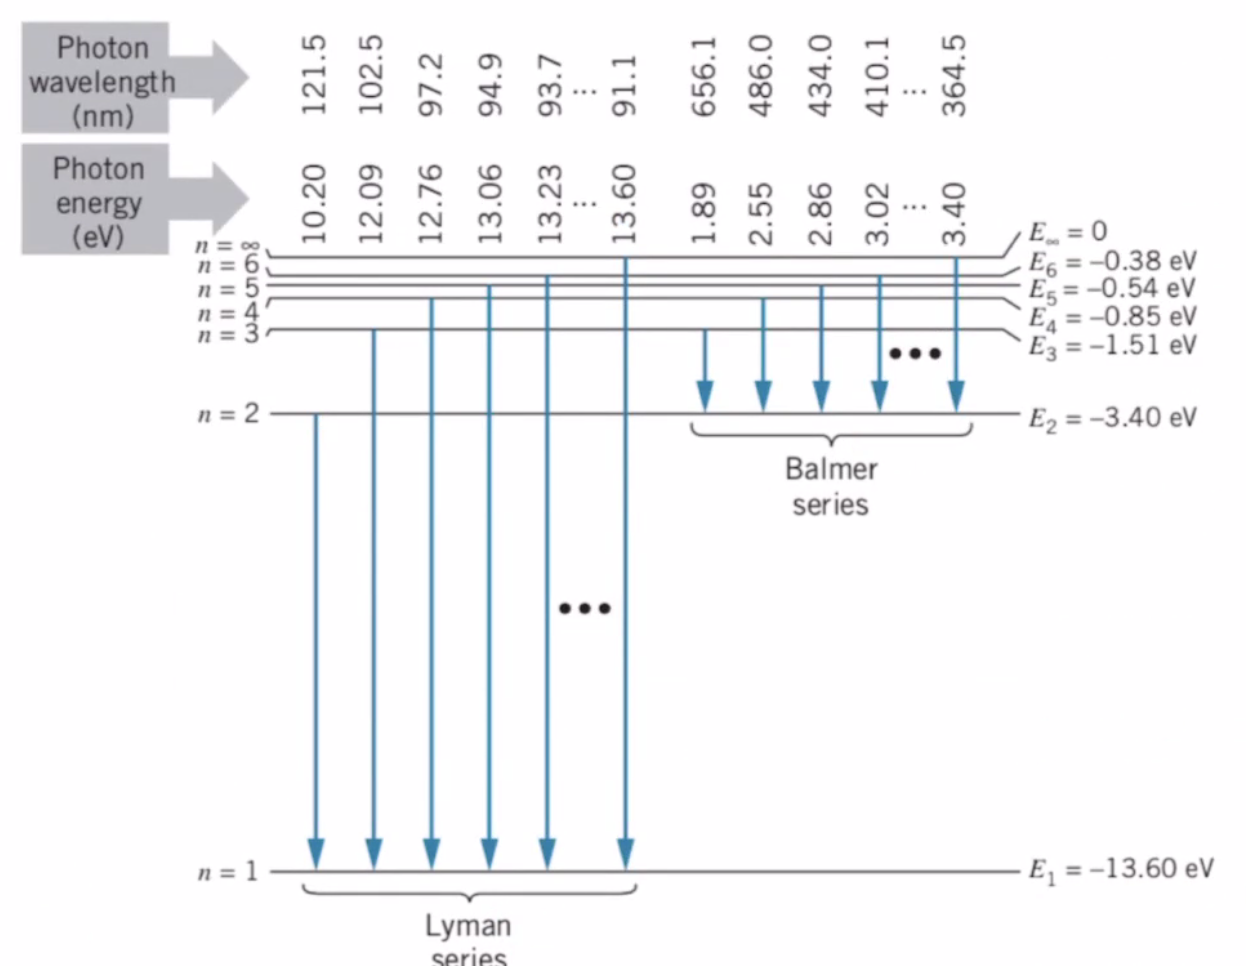
\includegraphics[width=.7\linewidth]{./Images/hydrogen_atom.png}
	\caption{This explains the difference between the emission and absorption spectra}
\end{figure}

If you have an excited energy, there are many possible emissions possible. However, if you excite an atom it is generally going to be completely in the ground state, so the absorption spectra has only one possibility.

\subsubsection{Borh model also explains}
\begin{enumerate}
\item Ritz combination principle\\
	\begin{itemize}
		\item Since frequency of an emitted photon is E=hf, summing
		\item
		\item
	\end{itemize}
\end{enumerate}

\begin{enumerate}
\item Ritz combination principle\\
	\begin{itemize}
		\item
		\item
		\item
	\end{itemize}
\end{enumerate}

\newpage
\subsubsection{Caveats}
Bohr can only work for atoms with a single electron. 
\[ Allowed\ radii: r_n = \frac{e_0n^2}{Z} \]
Z: \# positive charges,\\
He : Z = 2, ... \\
\\

Allowed energies:
\[E_k = (-13.60 eV) \frac{Z^2}{n^2} \]

\subsection{Franck-Hertz Experiment}
Illustrates the transition between different levels well. 

\begin{figure}[h]
	\centering
	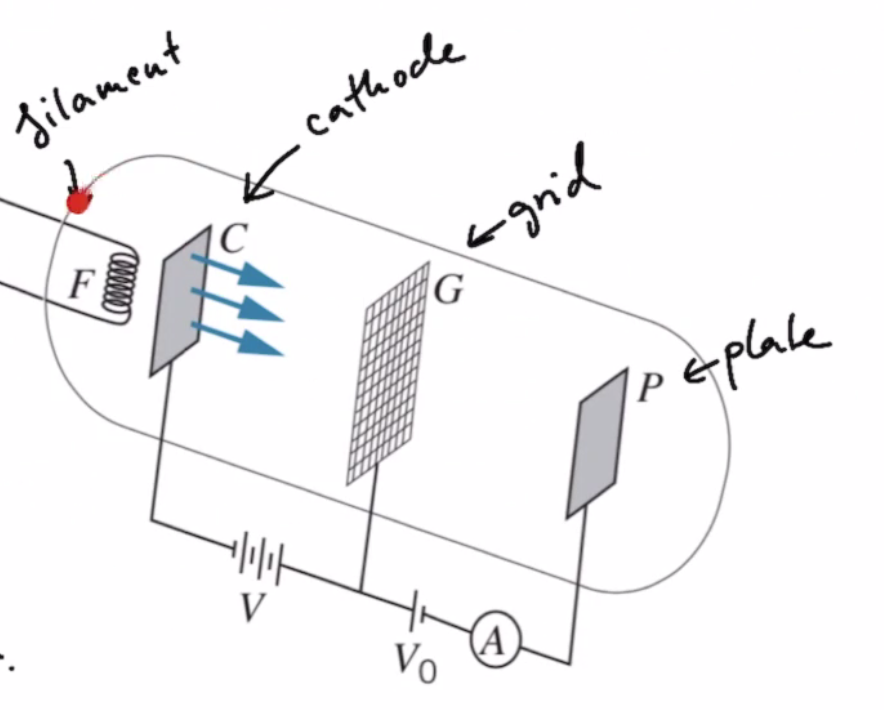
\includegraphics[width=.7\linewidth]{./Images/franck-hertz.png}
	\caption{Filament heats cathode, emits electrons that are accelerated using a voltage difference V. After passing grid, they are slowed by a retarding potential $V_0$}
\end{figure}

Filled the tube with mercury vapor.

\begin{figure}[h!]
	\centering
	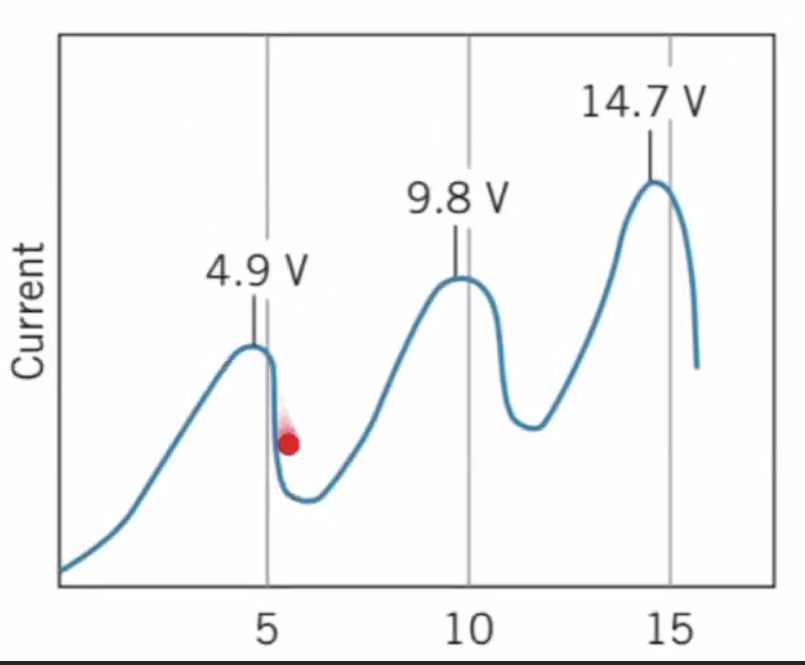
\includegraphics[width=.7\linewidth]{./Images/franck-hertz-results.png}
	\caption{Results meant that at some point the electron will have enough energy to excite one atom, and then eventually another atom.}
\end{figure}


\section{Wave-like properties of particles}
A natural extension of the behaviour of photons to other particles.

\subsection{De Broglie Wavelength}
Proposed that there is a wave with wavelength $\lambda$ associated to any matter particle moving with momentum p:
$$ \lambda = \frac{h}{p} $$
Where\\
h: Planck's constant\\
$\lambda$: de Broglie wavelength\\

Note that because planck's constant is so small, this is only really observable in tiny particles.\\
\\
This kind of came out of nowhere, but it turned out to be supported by evidence.\\

\begin{question}[Example]
	10g bullet travelling at 100 m/s
	\begin{answer}[Macroscopic object]
		$$\lambda = \frac{h}{p} = \frac{6.6 \cdot 10^{-34} J \cdot s}{0.010 kg \cdot 100 m/s} = 6.6 \cdot 10^{-34} m$$
	\end{answer}

	An electron ($m=0.511 MeV/c^2$) with kinetic energy 100 MeV
	\begin{answer}[Subatomic object]
		Kinetic energy $>>$ rest energy, we are in the extreme relativistic regime, so we can assume that the rest energy doesn't matter.\\
		$$ \lambda = \frac{h}{p} = \frac{hc}{pc} = \frac{1240 MeV \cdot fm}{100 MeV} = 12.4 fm = 1.24 \cdot 10^{-14} m $$
	\end{answer}
\end{question}

Why were wave-like properties of particle not observed previously? \\
\begin{itemize}
	\item For macroscopic objects, the wavelength is miniscule
	\item No experiment can be done to measure 
\end{itemize}

\newpage
\subsection{Diffraction Experiments}

\begin{figure}[h!]
	\centering
	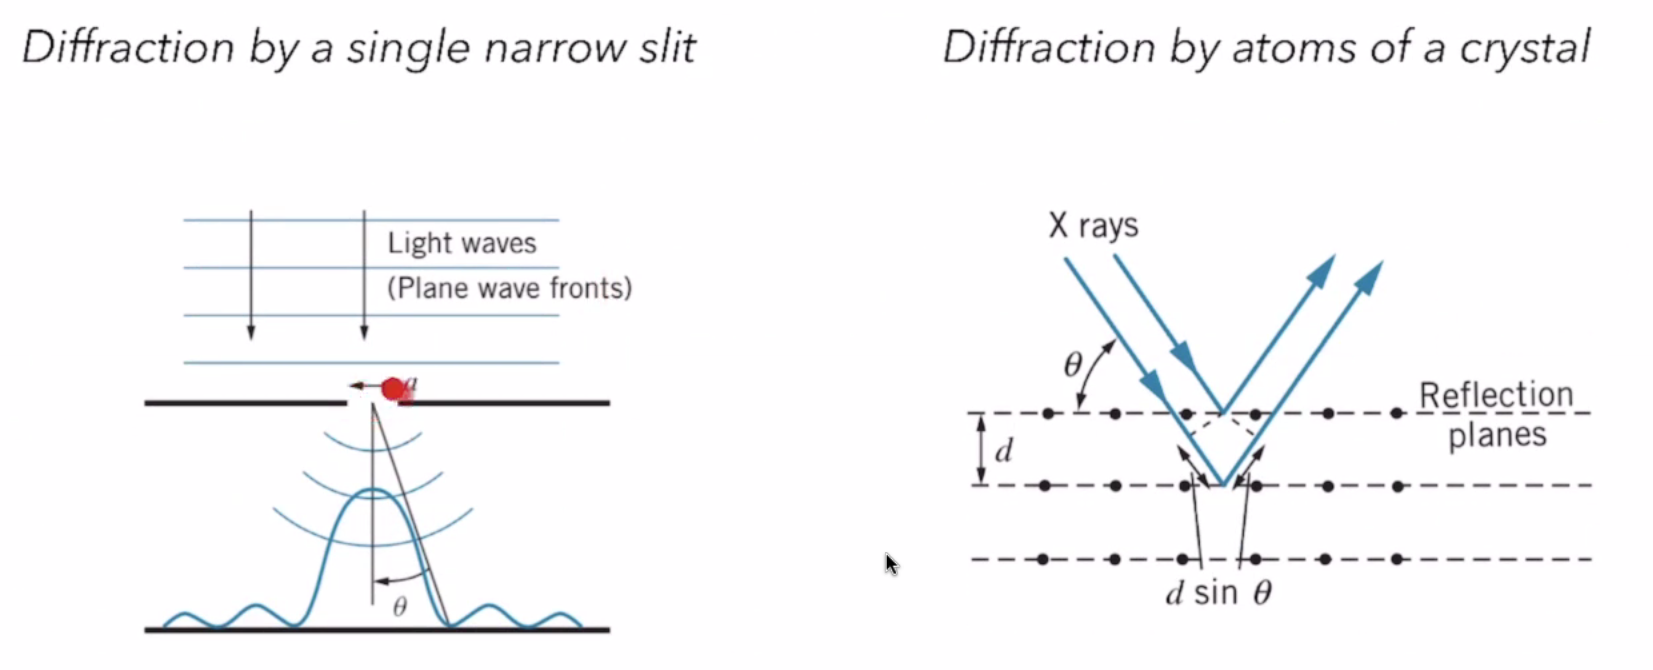
\includegraphics[width=.8\linewidth]{./Images/diffraction.png}
	\caption{}
\end{figure}

\subsubsection{Davisson-Germer Experiment}
First experiment verifying de Broglie's hypothesis. Investigated pattern of scattering electrons by surface of a crystal - which were found to display a typical diffraction pattern. 

\begin{figure}[h!]
	\centering
	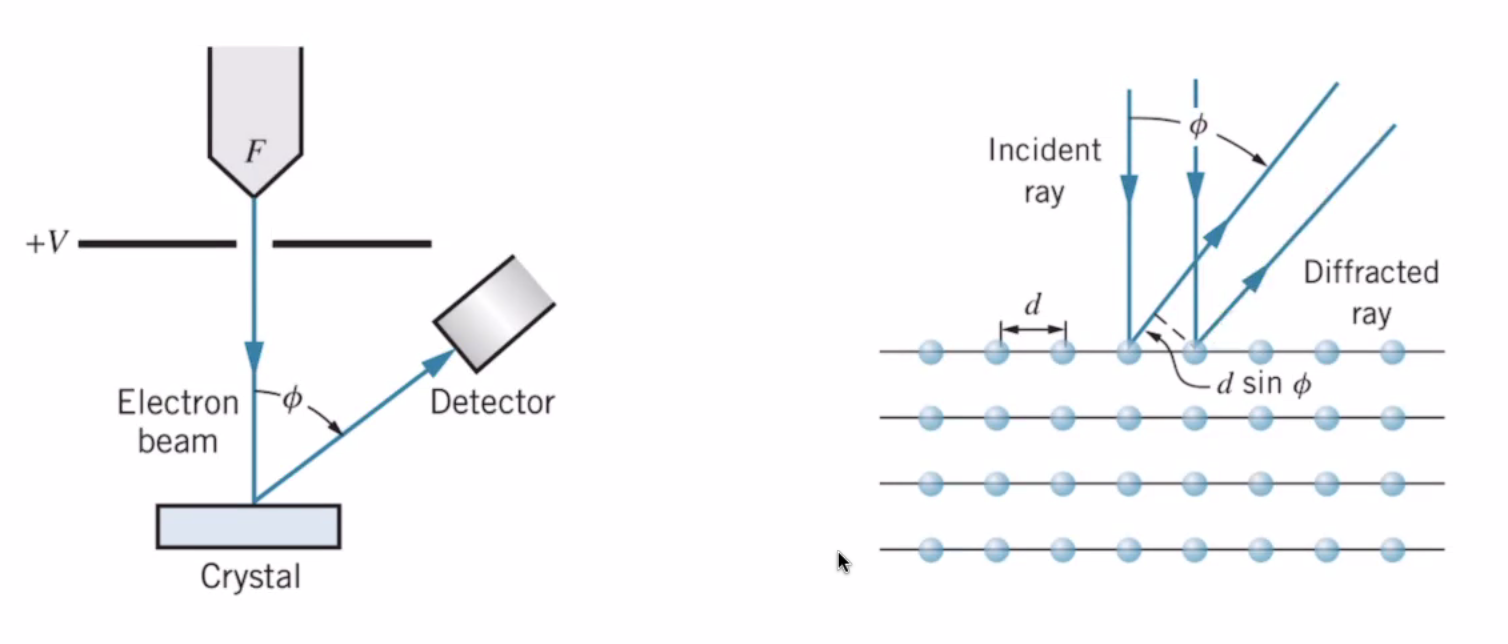
\includegraphics[width=.8\linewidth]{./Images/davisson.png}
	\caption{Similar patterns were found regardless of x-rays or electrons were used!}
\end{figure}


\begin{figure}[h!]
	\centering
	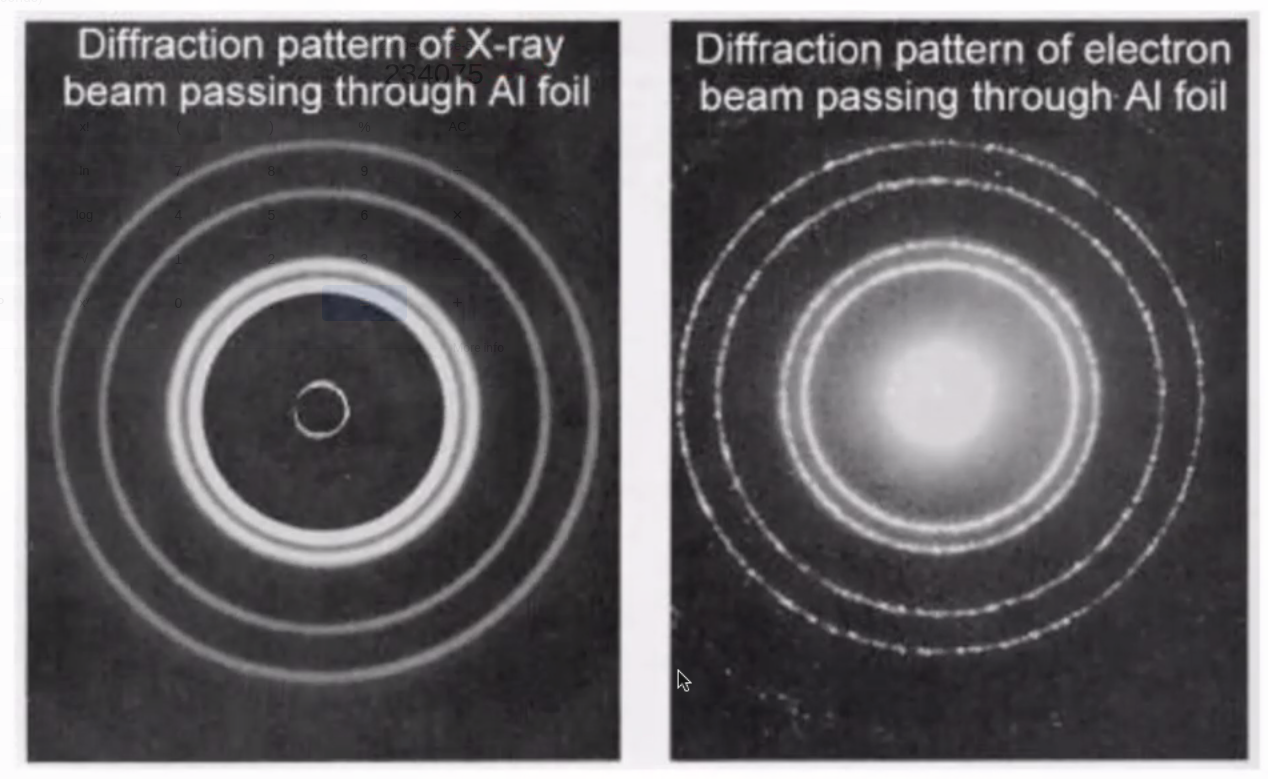
\includegraphics[width=.8\linewidth]{./Images/patterns.png}
	\caption{Polycrystaline material, shown for both photons and electrons}
\end{figure}

These similarities between diffraction patterns strongly suggested electrons are behaving like waves in these experiments. However, not just electrons can be used - any particle with a momentum has a de Broglie wavelength.

\subsection{Double-Slit Experiments}
First double-slit experiemtn with electrons was done first in 1961 (as numerous technological challenges had to be overcome).

\begin{figure}[h!]
	\centering
	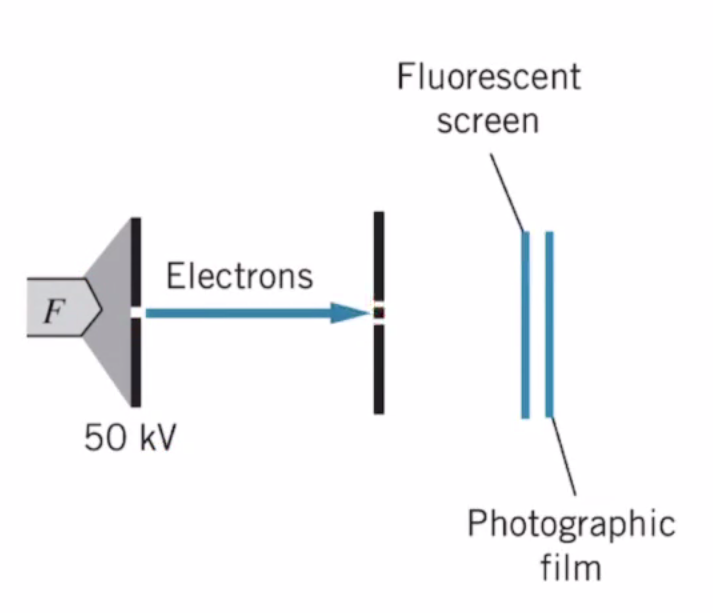
\includegraphics[width=.8\linewidth]{./Images/electron_doubleslit.png}
	\caption{Slit spacing of 2 $\mu$m, width 0.5 $\mu$m. An interference pattern was observed!}
\end{figure}

\newpage
\subsubsection{Electron Microscope}

A major advancement that this caused was the electron microscope. \\
It uses electron waves rather than visible light to illuminate and make images of objects. \textbf{\emph{Why?}} The wavelength can be made much shorter than those of visible light (and shorter than x-rays). \\

They can therefore be used for many purposes, e.g. in biomedical research. \\

\subsection{More Double-Slit}
Experiment with electrons passing through double-slits one at a time, slowly building up an interference image. \\

\begin{figure}[h!]
	\centering
	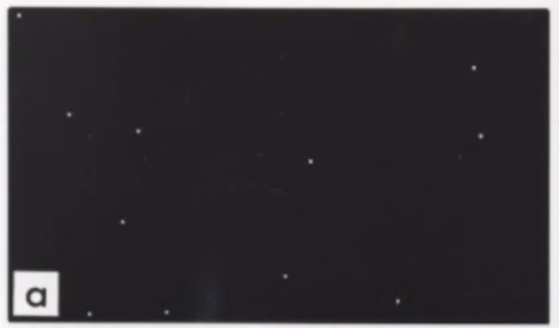
\includegraphics[width=.6\linewidth]{./Images/wave1.png}
	\caption{11 electrons}
\end{figure}

Even though the electrons are passing through one at a time, it seems somehow as though each electron is passing through both slits and is interfering with itself???\\

\begin{result}[Principle of Complementarity]
	The elctron (and other particles) behaves as a particle or a wave, but we cannot observe both aspects of its behavior simultaneously.\\
	A complete description of a photon/electron/particle cannot be made in terms of only particle properties or only wave properties. Both must be considered. The type of behavior we observe depends on the experiment we do!
\end{result}

\subsection{Uncertainty Principle}
\subsubsection{Classical Case}
For a particle, we will waant to know its position and momentum. \\
For a quantum particle, we will see that there are tradeoffs between these.\\

Waves and wave packets - \\
A pure sinusoidal wave extends from negative to positive infinity. This cannot describe a particle. Real waves are rather represented by ``wave packets", disturbance localized into a small region of space. \\

Uncertainty around measuring wavelength for a classical wave:\\

Uncertainty:
$$ \Delta \lambda \approx \epsilon\lambda (\epsilon\ around\ 10\%) $$

Size of disturbance:
$$ \Delta x \approx \lambda $$

Produce of these:
$$ \Delta \lambda \Delta x \approx \epsilon \lambda^2 $$


\begin{figure}[h!]
	\centering
	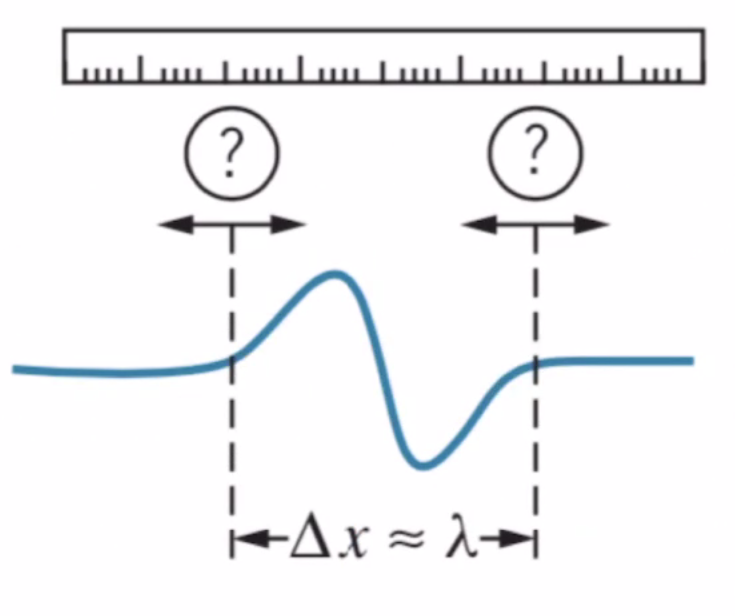
\includegraphics[width=.4\linewidth]{./Images/wave2.png}
	\caption{Uncertainty regarding where the wave begins and ends.}
\end{figure}


Try to make a larger wave packet:

\begin{figure}[h!]
	\centering
	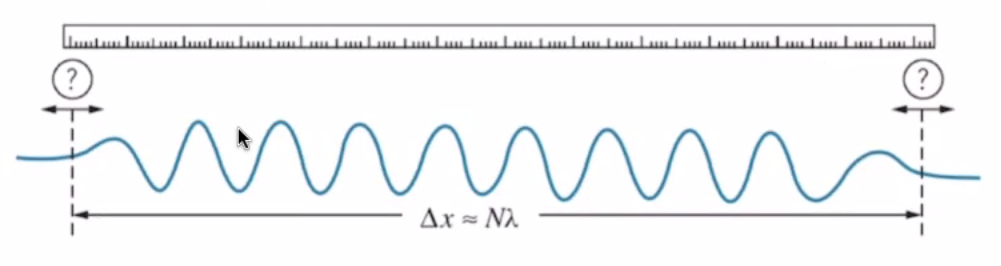
\includegraphics[width=.7\linewidth]{./Images/wave3.png}
	\caption{Uncertainty regarding where the wave begins and ends.}
\end{figure}
We now have N cycles of wave $\Delta x \approx N\lambda$. But we still have some uncertainty for start/end: $\epsilon x$. If we want to find the wavelength: $$\Delta x \approx \frac{\epsilon\lambda}{N}$$\\

Same product as before:
$$ \Delta x \Delta \lambda \approx N\lambda \frac{\epsilon \lambda}{N} = \epsilon \lambda^2 $$

\newpage
\begin{question}[Water waves]
	We are measuring wavelength of water waves and count 10 waves in a distance of 196 cm. What is the minimum uncertainty on the wavelength from this measurement?
	\begin{answer}[Answer]
		Wavelength:
		Wavelength: $ \lambda = \frac{196 cm}{N} = 19.6 cm $\\
		Uncertainty: $\epsilon = 1\% < \epsilon < 100\% \rightarrow \epsilon \approx 10\%$\\
		Uncertainty in measured wavelength:
		$$ \Delta \lambda \approx \frac{\epsilon \lambda^2}{\Delta x} = \frac{0.1 \cdot (19.6)^2}{196 cm} = 0.196 cm $$

	\end{answer}
\end{question}

\subsubsection{Heisenberg Uncertainty Relationships}
We can apply the uncertainty relationships (which apply to all waves) specifically to de Broglie waves.
$$ de\ Broglie\ wavelength: \lambda = \frac{h}{p} $$
It turns out that:
$$ \Delta x \Delta p_x \geq \frac{\bar{h}}{2} $$
Uncertainty in position times uncertainty in momentum is greater than pi times Planck's constant.\\
\\

Similarly:
$$ \Delta y \Delta p_y \geq \frac{\bar{h}}{2} $$
$$ \Delta z \Delta p_z \geq \frac{\bar{h}}{2} $$

We sometimes assume that this product is just equal to hbar.

\newpage
\begin{question}[Electron moves]
	An electron moves in the x direction with a speed of 3.6 $\cdot 10^6$ m/s. We can measure its speed with a precision of 1\%. With what precision can we simultaneously measure its x coordinate?
	\begin{answer}[Answer]
		Electron's momentum:
		$$ p_x = mv_x $$
		$$p_x = (9.11 \cdot 10^{-31} kg)(3.6 \cdot 10^6 m/s) = 3.3 \cdot 10^{-24} kg\ m/s $$
		Uncertainty on the momentum:
		$$ \Delta p_x = 0.01 \cdot p_x $$
		Uncertainty on the position:
		$$ \Delta x \geq \frac{\bar{h}}{2\Delta p_x} = \frac{1.05 \cdot 10^{-34} J \cdot s}{2 \cdot 3.3 \cdot 10^{-26}} kg \cdot m/s $$
		$$ \Delta x \geq 1.6 nm $$
		This uncertainty is actually several atoms large, which is pretty massive compared to the size of an electron itself.
	\end{answer}
\end{question}

\subsection{Heisenberg's Uncertainty Principles}
The quantum mechanical limit to the uncertainty of certain measurements, which results from
\begin{itemize}
	\item Wave-particle duality
	\item The interaction between what is observed and the observing instrument
\end{itemize}

\begin{result}[Uncertainty Principle]
	\begin{enumerate}
		\item
	\[ \Delta x \Delta p_x \geq \frac{\bar{h}}{2} \]
	$\bar{h} = 1.05 \cdot 10^{-34} J\cdot s $ \\
	$ = 6.58 \cdot 10^{-16} eV \cdot s$
		\item
	$$\Delta E \Delta t \geq \frac{\bar{h}}{2} $$
	It is not possible to make a simultaneous determination of the energy and the time coordinate of a particle with unlimited precision.
	\end{enumerate}
\end{result}

There is a second, similar relationship associated with the energy of the wave packet and the time taken to measure that energy. Consider that we have an uncertainty in the measured position of an object of $\Delta x$, which has a corresponding uncertainty for time traveled by the photon $\Delta t \approx \frac{\Delta x}{c}$. The uncertainty in energy is therefore\\
$$ \Delta E \approx \Delta p \cdot c $$


\begin{question}[Example]
	A) A charged pi meson has a rest energy of 140 MeV and a lifetime of 26 ns. What is the energy uncertainty of the pion? \\
	B) What about for a rho meson (rest energy of 765 MeV, lifetime of $4.4 \cdot 10^{-24} s$)?\\

	\begin{answer}[A]
		Using Heisenberg's second uncertainty principle, since we only have a limited amount of time to measure the energy.
		$$ \Delta E \geq \frac{\bar{h}}{2\Delta t} = \frac{6.58 \cdot 10^{-16} eV \cdot s}{2 \cdot 26 \cdot 10^{-9} s} = 1.3 \cdot 10^{-8} eV $$
		$$ \frac{\Delta E}{E} = \frac{1.3 \cdot 10^{-14} MeV}{140 MeV} \approx 10^{-16} $$
		This is a very small fractional error.
	\end{answer}
	\begin{answer}[B]
		$$ \Delta E \geq \frac{\bar{h}}{2\Delta t} = \frac{6.58 \cdot 10^{-16} eV \cdot s}{2 \cdot 4.4 \cdot 10^{-24} s} \approx 7.5 \cdot 10^{7} eV $$
		$$ \frac{\Delta E}{E} = \frac{7.5 \cdot MeV}{765 MeV} \approx 10\%$$
		For very short-lived particles, we cannot directly measure this lifetime. Instead, we can deduce the lifetime from the width/spread in the distribution of its rest energy.
	\end{answer}
\end{question}

\newpage
\begin{question}[Example]
	A ball of mass 50 g moves with a speed of 30 m/s. If its speed is measured to an accuracy of 0.1\%, what is the minimum uncertainty in its position?
	\begin{answer}[Answer]
		Momentum of ball:
		$$p_x = mv_x = 0.05 kg \cdot 30 m/s = 1.5 kg \cdot m/s $$
		Uncertainty in momentum:
		$$ \Delta p_x = 0.0015 kg \cdot m/s $$
		Minimum uncertainty in position:
		$$ \Delta x \geq \frac{\bar{h}}{2\Delta p_x} = \frac{1.05 \cdot 10^{-34} J \cdot s}{2 \cdot 0.0015 kg \cdot m/s} = 3.5 \cdot 10^{-30} m $$
		What does this mean?\\
		A typical nucleus of an atom is -15 to -14 m in the order of magnitude. \\
		The uncertainty here is roughly 16 orders of magnitude smaller.
	\end{answer}
\end{question}

\subsection{Difraction Experiment and Uncertainty Principle (and you!)}


\begin{figure}[h!]
	\centering
	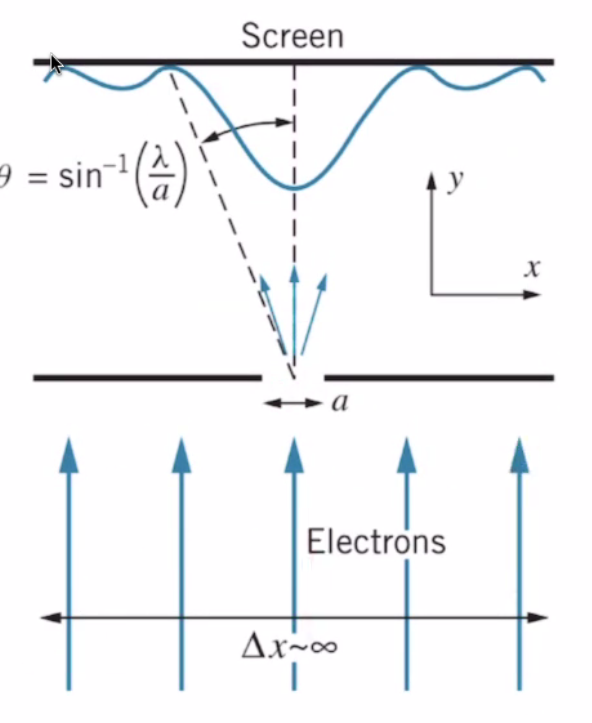
\includegraphics[width=.2\linewidth]{./Images/diff_unc.png}
	\caption{Incident electrons pass through a slit}
\end{figure}

Incident electrons moving in the y-direction with no component of momentum in the x-direction:
$$ p_x = 0, \Delta p_x = 0 \rightarrow \Delta x = \infty $$

Once electrons pass through the slit:
$$ \Delta x = a \rightarrow \Delta p_x \geq \frac{\bar{h}}{2 \Delta x} = \frac{\bar{h}}{2a} $$

Passing through slit means they acquire momentum component in x-direction!?! \\

Where on the screen would electron with this minimum momentum end up?
$$p_y = \frac{h}{\lambda} $$
For small angles $tan \theta \approx sin\theta \approx \theta$, so 
$$ \theta \approx \frac{p_x}{p_y} = \frac{\frac{h}{2\pi a}}{h/\lambda} = \frac{\lambda}{2\pi a} $$
For this diffraction experiment, minima described as:
$$ a \cdot sin\theta = h\lambda\ (n=1,2,3) $$

First minimum larger than spread of angles into which most particles diffracted. The distribution of transverse momentum roughly similar to the spread of the beam into the central diffraction peak. \\

The narrower the slit, the larger the uncertainty in momentum in x-direction is and the more the beam is spread out. \\

In a sense, understanding the diffraction experiment is a matter of the wave-like nature of particles, but looking at the central distribution is a matter of the particle nature.\\


\subsection{Wave Packets}
A wave associated with a particle is going to be a localized wave, a wave pulse or group, of limited spatial extent.\\

\subsubsection{Wave Group}
A wave group is a superposition of waves with different $\lambda$s, adjusted such that waves interfere constructively over a small region of space. Outside of this, they interfere destructively to zero amplitude everywhere. A physical phenomena to think of which is similar in concept is a beat. 

\subsubsection{Forming Wave Packets}
Key to forming wave packets is adding waves of different wavelength. Adding a small number gives more pronounced regions of large amplitude, but would still repeat from negative to positive infinity.\\ \\

Indeed, \emph{any finite combination of waves with discrete wavelengths will produce patterns that repeat from negative to positive infinity.}\\

Side note: Static wave vs traveling wave.\\
\emph{Static wave}: $y(x) = A cos(kx)$\\
\emph{Traveling wave}: $y(x, y) = A cos(kx - \omega t)$ \\
Where k is the wave number, $k = \frac{2pi}{\lambda}$, and $\omega$ is the angular frequency = $2\pi f$. \\

If we add two waves with a different wave number $k + \Delta k/2\ and\ k-\Delta k/2$, the resulting wave:
$$y(x, t) = A cos \left[(kt + \Delta k/2) x - (\omega + \Delta \omega/2)t \right] + A cos \left[ (kt - \Delta k/2) x - (\omega - \Delta \omega/2)t \right] $$
$$ = 2A cos \left( \Delta k/2 x - \Delta \omega / 2 \right) cos(kx - \omega t) $$

We define the speed of the wave packet, the group speed:
$$ v_g = \frac{\Delta \omega}{\Delta k} $$
\\

And the speed of the higher frequency wave within the group, phase speed (generally, phase speed is speed of a point of constant phase on the wave):
$$ v_p = \omega/k $$

We can generalize the group speed for more complicated wave packets as:
$$ v_g = \frac{d\omega}{dk} $$


\begin{question}[Group Velocity]
	Phase velocity of deep water waves ith a wavelength $\lambda$ is given by:
	$$ v_p = \sqrt{\frac{g\lambda}{2\pi}} $$ 
	Where g is the acceleration due to gravity. \\ \\

	Also, $v_p = \omega/k,\ \omega/k = \sqrt{g/k} \rightarrow \omega = \sqrt{gk} $\\
	Group velocity $v_g = \frac{d\omega}{dk} = \frac{d}{dk}(gk)^{1/2} = 1/2 \sqrt{g/k}$
\end{question}

\subsection{For de Broglie waves}
Energy of particle related to its frequency $ E = hf = \bar{h}\omega$ \\
Momentum of particle related to its wavelength $p = \frac{h}{\lambda} = \bar{h}k$ \\
Group speed of de Broglie wave:
$$ v_g = \frac{d\omega}{dk} = \frac{d E/\bar{h}}{dp/\bar{h}} = \frac{dE}{dp} $$
For classical particles with only kinetic energy:
$$ E = K + \frac{p^2}{2m} $$
$$ v_g = \frac{p}{m} = v $$

Which brings us back to where we started. The speed of a particle is equal to the group speed of the corresponding wave packet!


\section{Probabilities}
If we flip a coun can we predict the outcome? Similarly, in terms of systems govverned by the laws of quantum mechanics, we cannot predict the outcome of a single measurement of, e.g., position of an electron in an atom. However, if we do enough experiments we can find the statistical distribution. This is a fundamental aspect of nature and not a result of limited knowledge of the system we are studying.\\

\subsection{In matter particles, what is waving?}
The prbability of finding the particle at any point depends on the amplitude of its de Broglie wave at that point: Probability to observe particles $\propto |de\ Broglie\ wave\ amplitude|^2$. \\

\subsection{Wave function}
de Broglie waves are represented by wave functions: $\Psi(x,t),\ \Psi(x,y,z,t)$ \\

Wave functions are generally represented with complex numbers and used to calculate the probability of finding the particle at a given time in a small volume of space. \\

The probability that a particle will be found in the infinitesimal interval dx about the point x (P(x)dx) is: \\
$P(x)$: Probability density function
$$ P(x) \cdot dx = \left|\Psi(x,t)\right|^2dx$$

Complex wave function can be written as:
$$ \Psi = Re(\Psi) + i\ Im(\Psi) $$

The complex conjugate:
$$ z* = x-iy $$
$$ \Psi = Re(\Psi) - i\ Im(\Psi) $$

Squared magnitude of a complex number (or wave function) is the product of the numbver and its complex conjugate:
$$ |z|^2 = zz* = x^2 + y^2 $$
$$ |\Psi|^2 = \Psi \Psi* = Re(\Psi)^2 + Im(\Psi)^2 $$

Complex numbers are very useful in describing wave mechanics, in terms of amplitude and phases. Euler's formula expresses complex exponentials in terms of real trigonometric functions:
$$ e^{i\theta} = cos \theta + i\ sin \theta $$
$$ e^{-i\theta} = cos \theta - i\ sin \theta $$

Squared magnitude:
$$ |e^{i\theta}|^2 = e^{i\theta}e^{-i\theta} = e^0 = 1 $$
$$ |e^{i\theta}|^2 = (cos \theta + i\ sin \theta)(cos \theta - i\ sin \theta) = 1 $$

Trigonometric functions can be written in terms of complex functions as, e.g.:
$$ sin\theta = \frac{1}{2i} (e^{i\theta} - e^{-i\theta} $$
$$ cos\theta = \frac{1}{2i} (e^{i\theta} + e^{-i\theta} $$

\begin{result}[Wave function of a free particle]
	$$ \Psi(x,t) = Ae^{i(kx - \omega t)} = A \left( cos(kx - \omega t) + i sin(kx - \omega t) \right) $$
	k: wave number \\
	$\omega$: angular frequency \\
	$$ k = \frac{2\pi}{\lambda} = \frac{p}{\bar{h}} $$
	$$ \omega = 2\pi f - \frac{E}{\bar{h}} $$

	The probability function is given by
	$$ |\Psi(x,t)|^2 = A^2 $$
\end{result}



\subsection{Schrödinger Equation}
Basic equation of (non-relativistic) quantum mechanics.

Classical equivalent is Newton's second law:
$$ \vec{E} = \frac{d\vec{p}}{dt} $$

Schrödinger equation similarly written for a particle interacting with its environment but in terms of the potential energy rather than the force.\\

\subsection{Waves at Boundaries}
What happens to the wavelength and amplitude of a wave crossing from one region/medium to another?\\

\begin{figure}[h!]
	\centering
	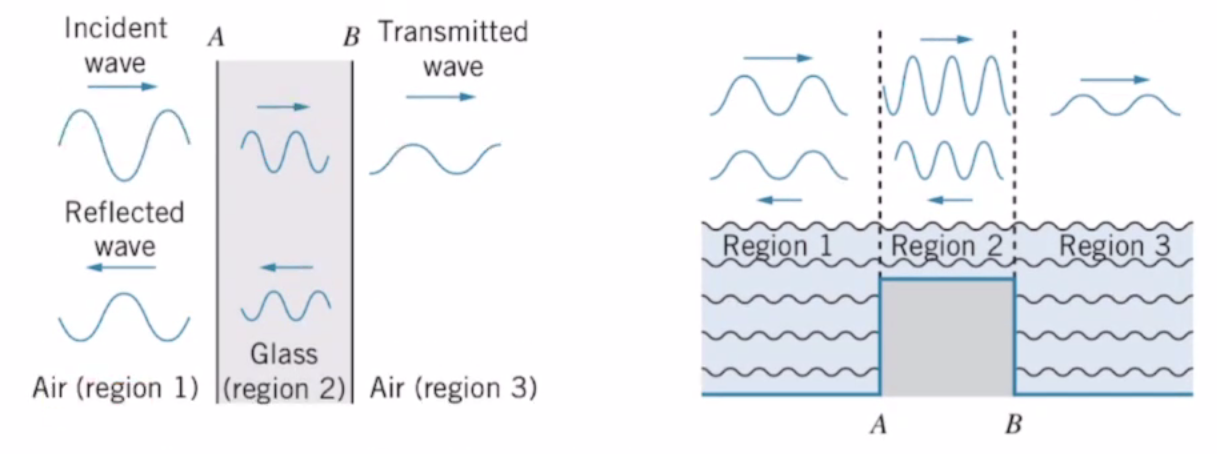
\includegraphics[width=.7\linewidth]{./Images/boundary.png}
	\caption{Similar behavior occurs for de Broglie waves - transmitted and reflected components!}
\end{figure}

Penetration of reflected wave:
\begin{itemize}
	\item For a fully reflected light wave, an ``evanescent wave" (exponentially decreasing) penetrates into the second medium.
	\item For de Broglie waves, these can also penetrate a short distance into the forbidden region though cannot be directly observed in that region.
	\item More on this (``tunneling") next week!
\end{itemize}

\subsubsection{Continuity at Boundaries}
When a wave crosses a boundary, two boundary conditions must be fulfilled.
\begin{enumerate}
	\item Wave function is continuous at the boundary
	\item Slope of wave function is continuous at the boundary, except when the boundary height is infinite (such as dropping a small metal ball onto a steel surface)
\end{enumerate}

\begin{figure}[h!]
	\centering
	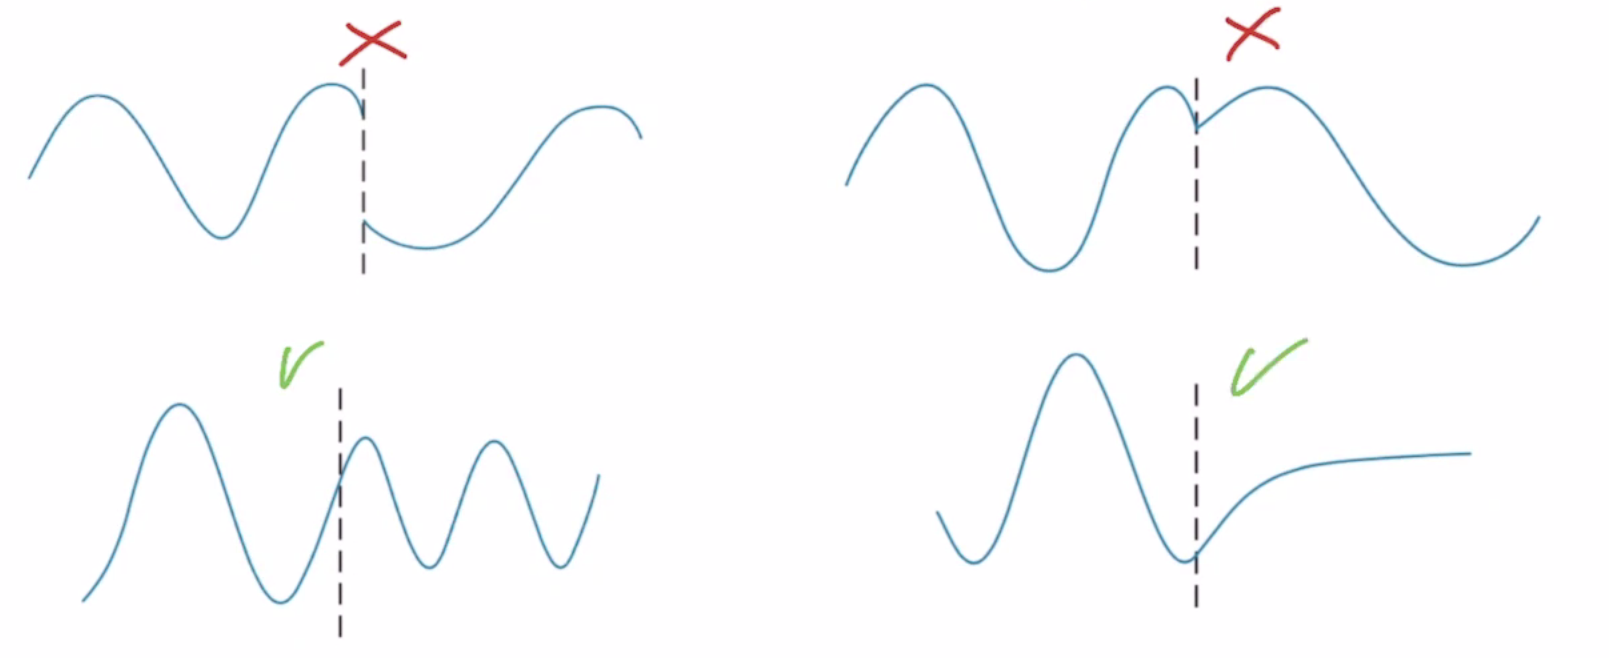
\includegraphics[width=.9\linewidth]{./Images/boundary-waves.png}
	\caption{Examples of invalid and valid wave phenomena at boundaries.}
\end{figure}

\subsection{Particle in a Potential Energy Well}

A free particle is by definition not confined - can be located anywhere, has definite wavelength, momentum, and energy.\\
A confined particle is instead represented by a a wave packet and can be found within a small region of space $\Delta x$ (e.g. electron confined in an atom)\\

\subsubsection{Finite Potential Barrier}

\begin{figure}[h!]
	\centering
	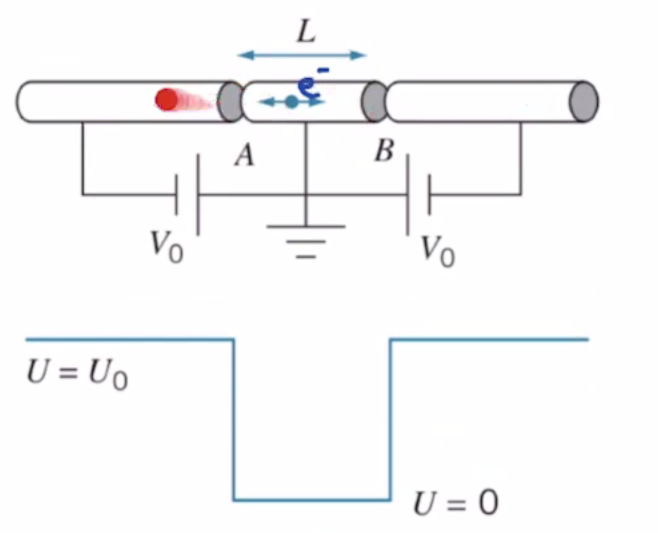
\includegraphics[width=.4\linewidth]{./Images/potential_well.png}
	\caption{Potential well}
\end{figure}

Potential energy:
$$ U_0 = qV = (-e)(-V_0) = eV_0 $$
If electron kinetic energy K is smaller than the potential energy $K < U_0$, the electron cannot overcome the potential confined in that region.
\newpage
\subsubsection{Infinite Potential Barrier}
Consider simplified scenario where the potential energy barrier at points A and B is infinitely high. 
\begin{itemize}
	\item Penetration into ``forbidden" region cannot occur
	\item Probability of waves find electron is exactly zero in those regions
	\item Wave function must be zero at boundaries A and B to be continuous
\end{itemize}


\begin{figure}[h!]
	\centering
	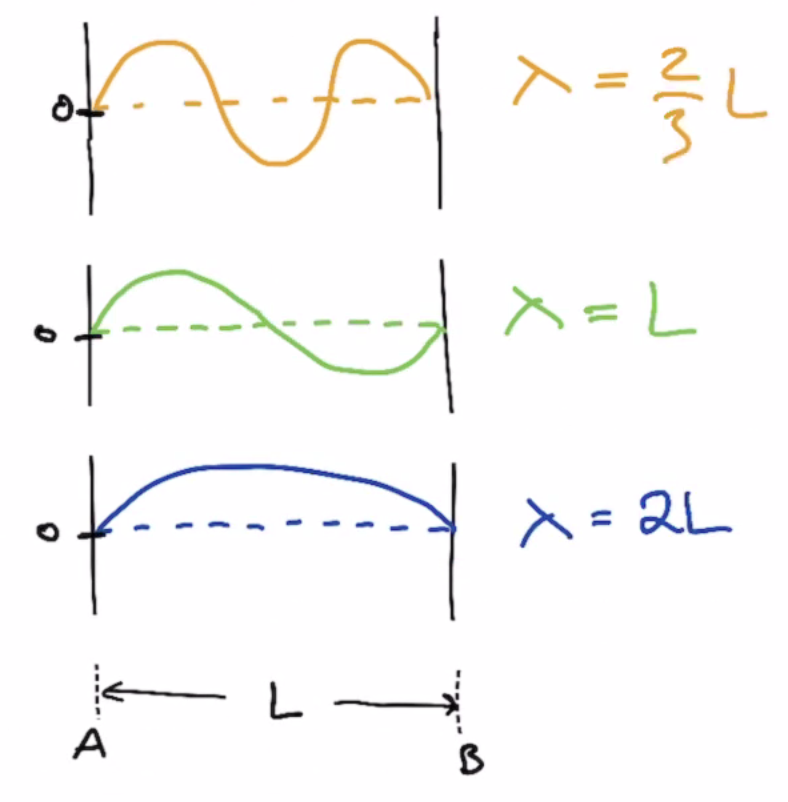
\includegraphics[width=.4\linewidth]{./Images/possible_waves.png}
	\caption{Possible waves and wavelengths that could describe this scenario}
\end{figure}

We see that only certain wavelengths are allowed.
$$ \lambda_n = \frac{2L}{n},\ n = 1,2,3... $$

This also means that only cetrtain momentua are allowed:
$$ p_n = n \frac{h}{2L}\ n = 1,2,3... $$

This also means that only cetrtain energies are allowed: \\
$ K = \frac{p^2}{2m} = E $ given that potential energy is zero.
$$ E_n = n^2 \frac{n^2}{8mL^2}\ n=1,2,3... $$

\emph{\textbf{Energies are quantized!}} \\

The classical version of this is, essentially guitars. \\

\begin{result}[On energy quantization]
	Any attempt to confine a particle to a finite region of space will result in quantization of energy.\\

	This is a core feature of quantum mechanics
\end{result}

\begin{question}[Model of an atom]
	We can approximate an atomic electron as confined in an infinite square well. Use this model to approximate the energy required to raise an atomic electron from the state n=1 to n=2, assuming the atom has a radius of 1 Á.
	\begin{answer}[Answer]
		Allowed energy
	\end{answer}
\end{question}


\subsection{Normalization of Wave Function}
For a particle along th ex-axis (one-dimensional), the patricle must be \emph{somehwere} along the x-axis and the probabilities summed over all values must add to exactly 1.
$$  \int_{-\infty}^\infty P(x,t)\ dx =  \int_{-\infty}^\infty |\Psi(x,t)|^2 dx = 1 $$

Any wave function satisfying this is said to be "normalized".\\

Similarly, probability of finding the particle in a finite interval $a \leq x \leq b$:
$$ Probability\ P = \int_a^b |\Psi(x,t)|^2\ dx $$

\begin{question}[Example]
	The initial (t=0) wave function for a particle is given by:
	$$ \Psi(x,0) = ce^{-|x|/x_0} $$

	\begin{answer}[Normalize the wave function]
		$$1 = \int_{-\infty}^\infty |\Psi(x,t)|^2\ dx = c^2 \int_{-\infty}^\infty e^{-2|x|/x_0} dx $$
		This integral is symmetric about the y axis. Simplify as 2x the integral from 0 to infinity.
		$$ 1 = 2 c^2 \int_{0}^\infty e^{-2|x|/x_0} dx = 2c^2\left[-\frac{x_0}{2} e^{-2x/x_0}\right]^\infty_0 = 2c^2(0 + \frac{x_0}{2} = c^2 x_0 $$
		$$ c = \sqrt{1/x_0} $$
	\end{answer}
	\begin{answer}[Probability of finding the particle on an interval]
		$$ P = \int_{-x_0}^{x_0} |\Psi(x,0)|^2 dx =c^2 \int_{-\infty}^\infty e^{-2|x|/x_0} dx $$
		$$ P = 2\frac{1}{x_0} \left( -\frac{x^0}{2} \right) \left[ e^{-2/x_0}\right] = (-1)(e^{-2} - 1) $$
		Approximately 0.865. Apparently has nothing to do with x0.
	\end{answer}

\end{question}

\section{The Schrödinger Equation}
The differential equation that describes the wave behavior of particles for non-relativistic motion.

\begin{result}[Time-Independent Version]
	$$ -\frac{\bar{h}^2}{2m} \frac{d^2\Psi}{dx^2} + U(x)\Psi(x) = E\Psi(x) $$
	$\Psi(x)$: Wave function describing particle at a particular time\\
	U(x): potential energy\\
	E: total non-relativistic energy of the particle\\
	m: mass of the particle \\
	$\bar{h}:\ \frac{h}{2\pi}$
	Note, this cannot be derived, it is motivated.
\end{result}

\subsection{Motivation of the time-independent form of the Schrödinger equation}
$$ -\frac{\bar{h}^2}{2m} \frac{d^2\psi}{dx^2} + U(x)\psi(x) = E\Psi(x) $$
If the latter two terms are potential and total energy, is the first term corresponding to kinetic energy? \\

$$ K = \frac{p^2}{2m} = \frac{(h/\lambda)^2}{2m} = \frac{(\bar{h}k)^2}{2m} $$
Note that this is sort of similar to the first part, the difference is if we divide this by $-k^2$ then it's the same as the first fraction in the first term of the Schrödinger equation.\\


For a wave function: $\Psi(x) = A sin(kx)$
$$ \frac{d\psi}{dx} = kA cos(kx) $$
$$ \frac{d^2\psi}{dx^2} = -k^2 A cos(kx) $$
Think of the first term as kinetic energy:
$$ k\psi(x) = -\frac{\bar{h}^2}{2m} \frac{d^2\psi}{dx^2} $$
\\

If we take potential energy as used in deriving the Bohr model:
$$ U(x) \rightarrow U(r) = -\frac{1}{4\pi\epsilon_0} $$

\subsection{Time-dependent Schrödinger equation}
This is sorta beyond the scope of the class.... but: \\
Wave function:
$$ \psi(x)\ vs\ \Psi(x,t) $$
$$ -\frac{\bar{h}^2}{2m} \frac{\delta^2\Psi}{\delta x^2} + U(x) \Psi(x,t) = i\bar{h} \cdot \frac{\delta\Psi}{\delta t} $$
$$ \Psi(x,t) = A e^{i(kx - \omega t)} $$
This new part:
$$ i\bar{h} \frac{\delta \Psi}{\delta t} = i\bar{h} A(-i\omega)e^{i(kx-\omega t)} = \bar{h} w \Psi(x, t) $$
Note the extra hbar omega.

$$\Psi(x,t) = \psi(x) e^{-i\omega t} $$
The last part is the time-independent part.

\subsection{Solving the Schrödinger Equation?}
\begin{enumerate}
	\item	Write down time-independent Schrödinger equation with the appropriate potential U(x), may need different expressions for different regions if U(x) changes discontinuously.
	\item 	Find wave function solution $\psi(x)$
	\item 	Apply boundary conditions (often more than one solution is found - applying boundary conditions help iliminate solutions), and continuity conditions (if applicable).
	\item 	Normalize the wave function.
	\item 	Since wave function (squared) represents a probability, any solution that becomes infinite must be discarded.
\end{enumerate}

From the wave function, we can calculate:
\begin{itemize}
	\item Probability to find the particle in an interval
	\item Outcome of a single measurement is not guaranteed, but we can determine the average of many measurements, e.g. of the position coordinate x of a particle:
		$ We\ measure: x_1,\ n_1,\ times,\ x_2,\ n_2,\ time.... $ \\
		Average: $x_{av} = \frac{x_1n_1 + x_2n_2 + ...}{n_1 + n_2 + ...} = \frac{\sum x_in_i}{\sum n_i} $\\
		In terms of probabilities: $P_1 = \frac{n_1}{N},\ ...$
		$$x_{av} = \sum x_iP_i $$
		Possible values are distributed continously - probability of finding particle in an infinitesimal range dx about point x is:
		$$ P(x)dx $$
		$$ Average: <x> = \int_{-\infty}^{\infty} x P(x)\ dx = ^{\infty} x |\Psi(x)|^2\ dx $$
		These $<x>$ are called expectation values.
\end{itemize}

\newpage
\subsection{Back to that Infinite Potential Well}

\begin{figure}[h!]
	\centering
	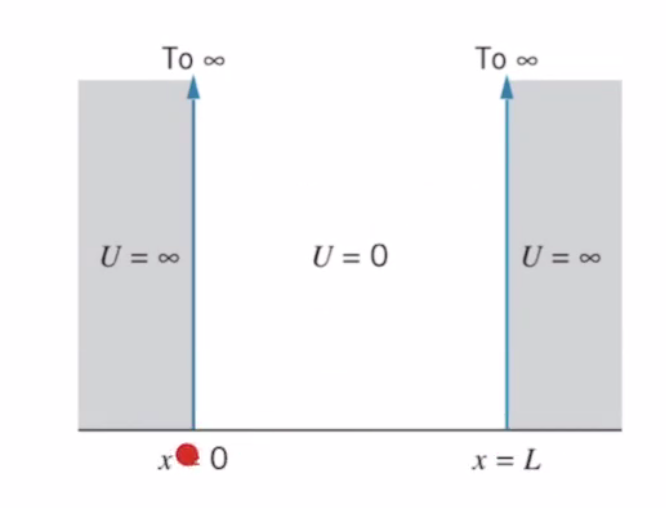
\includegraphics[width=.4\linewidth]{./Images/well.png}
	\caption{Infinite potential well}
\end{figure}
Potential energy can be expressed as:
$$ U(x) = 0\ for\ 0\leq x \leq L $$
$$ U(x) = \infty\ for\ x < 0, x > L $$

Wave function for region outside of well?\\
Probability of finding particle then must be zero everywhere:
$$\\si(x) = 0 $$ for $x < 0, x > L$\\

Schrödinger equation for region inside of well ($0 < x < L$):
$$ \frac{\bar{h}^2}{2m} \frac{d^2\psi}{dx^2} = E\psi(x) $$
General solution $\left( \frac{d^2\psi}{dx^2} \right) = constant \cdot \psi(x) $\\
$$ \psi(x) = A sin(kx) + Bcos(ks) $$
(for $0 \leq x \leq L$)
$$ \frac{d^2\psi}{dx^2} = -k^2 \psi(x) $$
$$ k^2 = \frac{2mE}{\bar{h}^2} $$
or:
$$ k = \frac{\sqrt{2mE}}{\bar{h}} $$
So what's up with those random constants A and B?\\
It has to do with the constraint that the wave function at the boundaries must be 0.
$$ 0 = \psi(0) = A sin(0) + B cos(0) = B \rightarrow B = 0 $$
$$ 0 = \psi(L) = A sin(kL) + B cos(kL) = A sin(kL) $$
$$ A sin(kL) = 0 $$
So A can't be 0 because then our wave function isn't useful. Therefore, $sin(kL) = 0$\\
$$kL = n\pi,\ (n=1,2,3,...) $$
$$ k = \frac{n\pi}{L} $$
Wavelength?
$$ \lambda = \frac{2\pi}{k} = \frac{2L}{n} $$
Same as yesterday! \\
\skip

We now have:
$$ \psi(x) = A sin\left(\frac{u\pi}{L} x\right)\ for\ 0 \leq x \leq L $$
What is A? Normalize!

$$ 1 = \int_{-infty}^\infty |\psi(x)|^2\ dx = A^2 \int_0^L sin^2\left(\frac{n\pi}{L} x\right)\ dx $$
Use $sin^2x = 1/2 (1-cos(2x))$.
$$ 1 = A^2 1/2 \int_0^L (1-cos\left(\frac{n\pi}{L} x\right))\ dx $$
$$ 1 = A^2 1/2 \left[x - \frac{L}{2n\pi} sin\left(\frac{2n\pi}{L} x\right)\right]^L_0 = \frac{A^2L}{2} $$
$$ A = \sqrt{\frac{2}{L}} $$

\begin{figure}[h!]
	\centering
	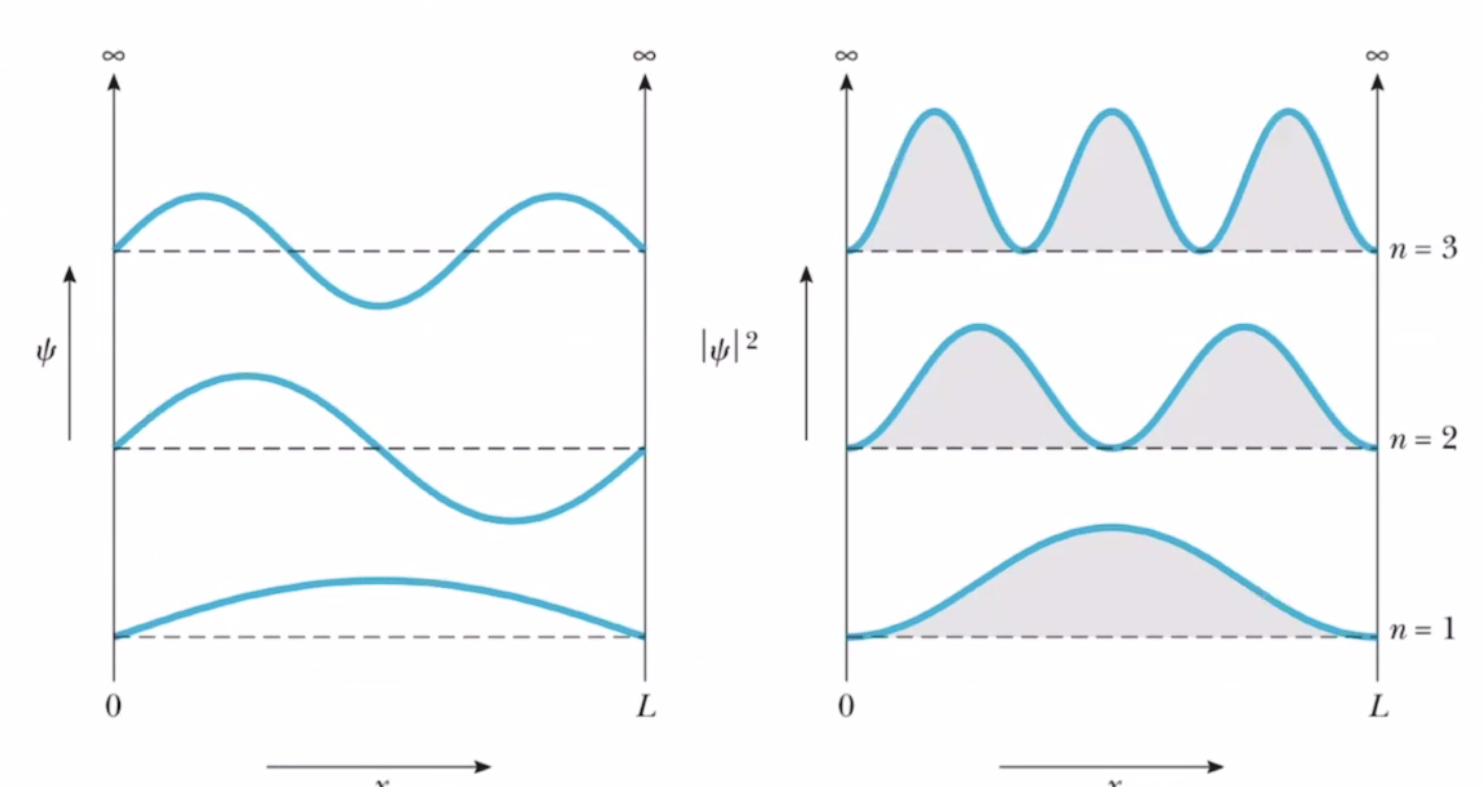
\includegraphics[width=.7\linewidth]{./Images/probability_or_function.png}
	\caption{We can look at the wave function and probability density for n=1,2,3}
\end{figure}

\subsection{Stationary States}
Solutions to the time-dependent Shrödinger equation that can be written as above are called \textbf{stationary states}. Their probability density does not depend on time, since:
$$ |\Psi(x,t)|^2 = |\psi(x)|^2\ |e^{-e\omega t}|^2 $$
$$ |e^{-e\omega t}|^2 = e^{-i\omega t} e^{+i\omega t} = 1 $$


In our course, we will restrict our discussion to stationary states and the time-independednt Schrödinger equation.

\begin{result}[Schrödinger Equation for Constant Potential Energy]
	Let's examine the Schrödinger equation when U(x) is constant. $U(x) = U_0$.
	$$ \frac{-\bar{h}^2}{2m}\frac{d^2\psi}{dx^2} + U_0 \psi(x) = E \psi(x) $$
	or:
	$$ \frac{d^2\psi}{dx^2} = -\frac{2m}{\bar{h}} (E - U_0) \psi(x) $$
	Right side of the equation is constant.
	Given $ E > U_0$
	$$ \frac{d^2\psi}{dx^2} = -k^2 \psi(x) $$
	$$ k = \sqrt{\frac{2m(E-U_0)}{\bar{h}^2}} $$
	General Solution:
	$$ \psi(x) = Asin(kx) + Bcos(kx) $$
	Since:
	$$ \frac{d\psi}{dx} = Ak cos(kx) - Bk sin(kx) $$
	$$ \frac{d\psi^2}{dx^2} = - Ak^2 cos(kx) - Bk^2 sin(kx) = -k^2 \psi(x) $$

	Given $ E < U_0$
	$$ \frac{d^2\psi}{dx^2} = (k')^2 \psi(x)$$
	$$ k' = \sqrt{\frac{2m(U_0 - E)}{\bar{h}^2}} $$
	General Solution:
	$$ \psi(c) = Ae^{k'x} + Be^{-k'x} $$
	Since:
	$$ \frac{d\psi}{dx} = Ak'e^{-k'x} - Bk'e^{-k'x} $$
	$$ \frac{d\psi}{dx} = A(k')^2e^{-k'x} - B(k')^2e^{-k'x} = (k')^2 \psi(x) $$
	\emph{This is the forbidden region}
\end{result}

\subsection{Schrödinger Equation for Free Particle}
Free particle implies no force acting upon it implies potential energy is constant. We can choose any value for that constant, but for simplicity we choose 0. \\

Schrödinger equation:
$$ -\frac{\bar{h}^2}{2m} \frac{d^2\psi}{dx^2} = E\psi(x) $$

We already determined the general solutions!
$$ \psi(x) = Asin(kx) + Bcos(kx) $$
$$ k = \sqrt{\frac{2m(E-U_0)}{\bar{h}^2}} $$

Or expressing energies (E) in terms of wave numbers (k):
$$ E = \frac{\bar{h}^2k^2}{2m} \left( = \frac{p^2}{2m} \right) \leftarrow Energy\ not\ quantized $$

Useful to express wave function as a complex exponential:
$$ Euler's\ formula:\ e^{ikx} = cos(kx) + i\ sin(kx)$$
$$ cos(xk) = \frac{e^{ikx} + e^{-ikx}}{2},\ \  sin(xk) = \frac{e^{ikx} - e^{-ikx}}{2i} $$

Substitute these in the expression for the wave function:
$$ \psi(x) = A\left(\frac{e^{ikx} + e^{-ikx}}{2}\right) + B\left(\frac{e^{ikx} - e^{-ikx}}{2i}\right) $$

$$ = A' e^{ikx} + B' e^{-ikx} $$ Where A' and B' are constants.

This was the time-independent part, we write teh complete time dependent wave function as:
$$ \Psi(x,t) = \psi(x) e^{-iwt} = A' e^{i(kx-\omega t)} + B' e^{-i(kx-\omega t)} $$
A term is a wave moving in the positive x direction, and the B term is a wave moving in the negative x direction.

\begin{question}[A Free Particle]
	Consider a free particle moving in the positive x direction - must set B' = 0.
	$$ \Psi(x,t) = A' e^{i(kx-\omega t)} $$

	\begin{answer}[Associated Probability Density]
		$$ P(x) = |\Psi(x,t)|^2 = |A'|^2 e^{i(kx - \omega t)} e^{-i(kx - \omega t)} \rightarrow \ The \ e\  terms\  cancel\  out\ \rightarrow |A'|^2 $$
		This is a constant!
	\end{answer}
\end{question}

\subsection{Finite Potential Energy Well}
Previously we considered separately the solutions for inside/outside an infinite potential well and the resulting boundary conditions. This lead to quantization of energy. \\

This infinite potential well rests on assumptions we can't live with! \\

Potential energy:
$$ U(x) = 0\ for\ 0\leq x\leq L $$
$$ U(x) = U_0\ for\ x < 0 x > L $$

We will sconsider separately regions inside and outside. \\
Inside well, the same general wave function solution:
$$ \psi(x) = A sin(kx) + B cos(kx) $$
Where 
$$ k = \sqrt{\frac{2mE}{\bar{h}^2}} $$
We need those A and B constants at some point. \\

Now, outside of the well, particle is confined (energy is less than the potential energy):
$$ (E < U_0): \psi(x) = C e^{k'x} + De^{-k'x} $$
$$ k' = \sqrt{\frac{2m(U_0 - E)}{\bar{h}^2}} $$
We need those C and D constants at some point. \\

Now, let's consider separately the regions $x < 0\ and\ x > L$:
$$ x < 0:\ As\ x \rightarrow -\infty = \psi(X) = Ce^{k'x} $$
As D would approach infinity so we can't have that.
$$ x > L:\ As\ x \rightarrow \infty = \psi(X) = De^{-k'x} $$
As C would approach infinity so we can't have that. \\

In summary, we have found for the finite potential energy well:\\
\begin{align*}
	\psi(x) = C e^{k'x} & \ for\ x < 0 \\
	\psi(x) = A sin(kx) + B cos(kx) & \ for\ 0 \leq x \leq 0 \\
	\psi(x) = D e^{-k'x} & \ for\ x > L 
\end{align*} \\
We have a lot of equations for a lot of unknowns, and solving is quite hard.

\begin{figure}[h!]
	\centering
	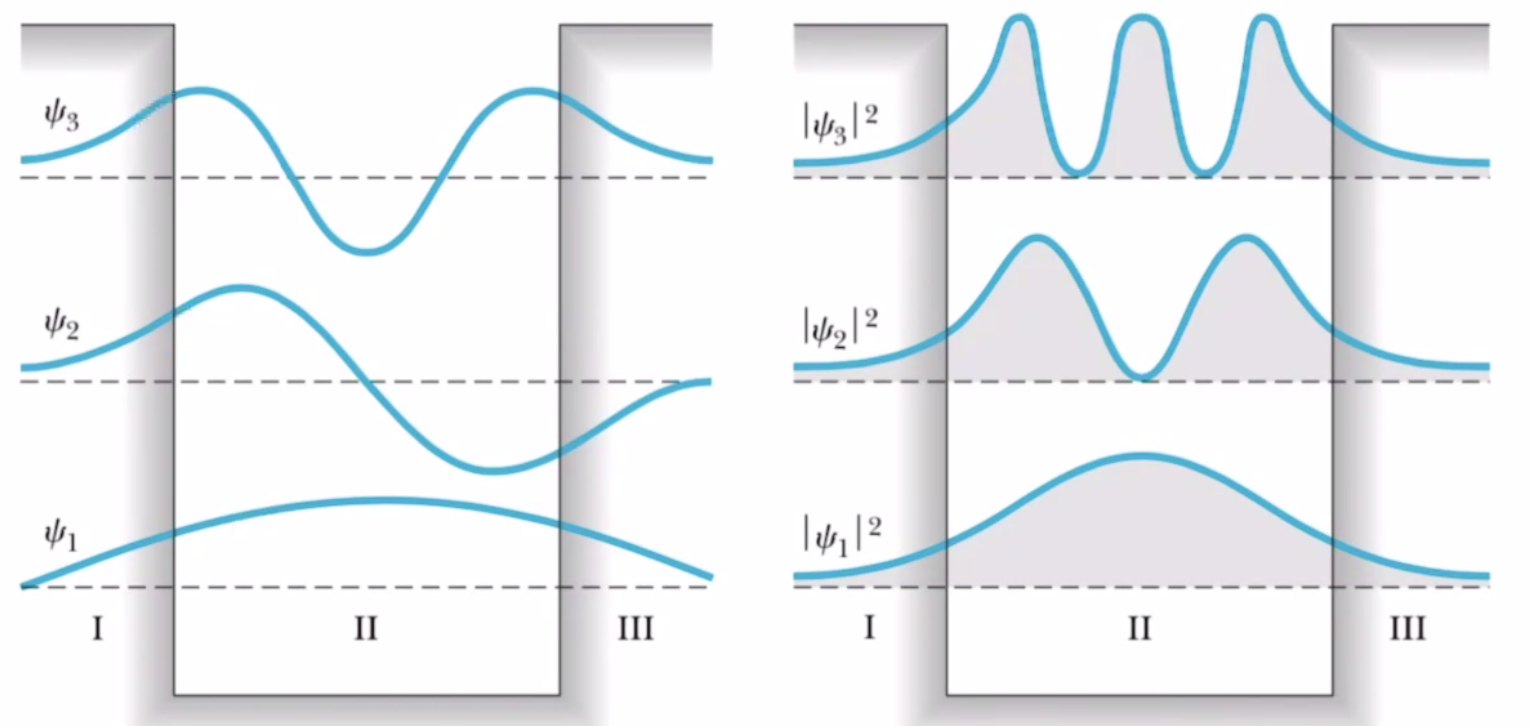
\includegraphics[width=.9\linewidth]{./Images/three_lowest.png}
	\caption{Note how the probability outside the finite potential energy well is NOT zero!!}
\end{figure}



\end{document}
